\section{Introduction}

\subsection{History}

\begin{frame}
  \frametitle{From birth to early successes (1940--1974)}

  \begin{textblock}{100} (0,10)
    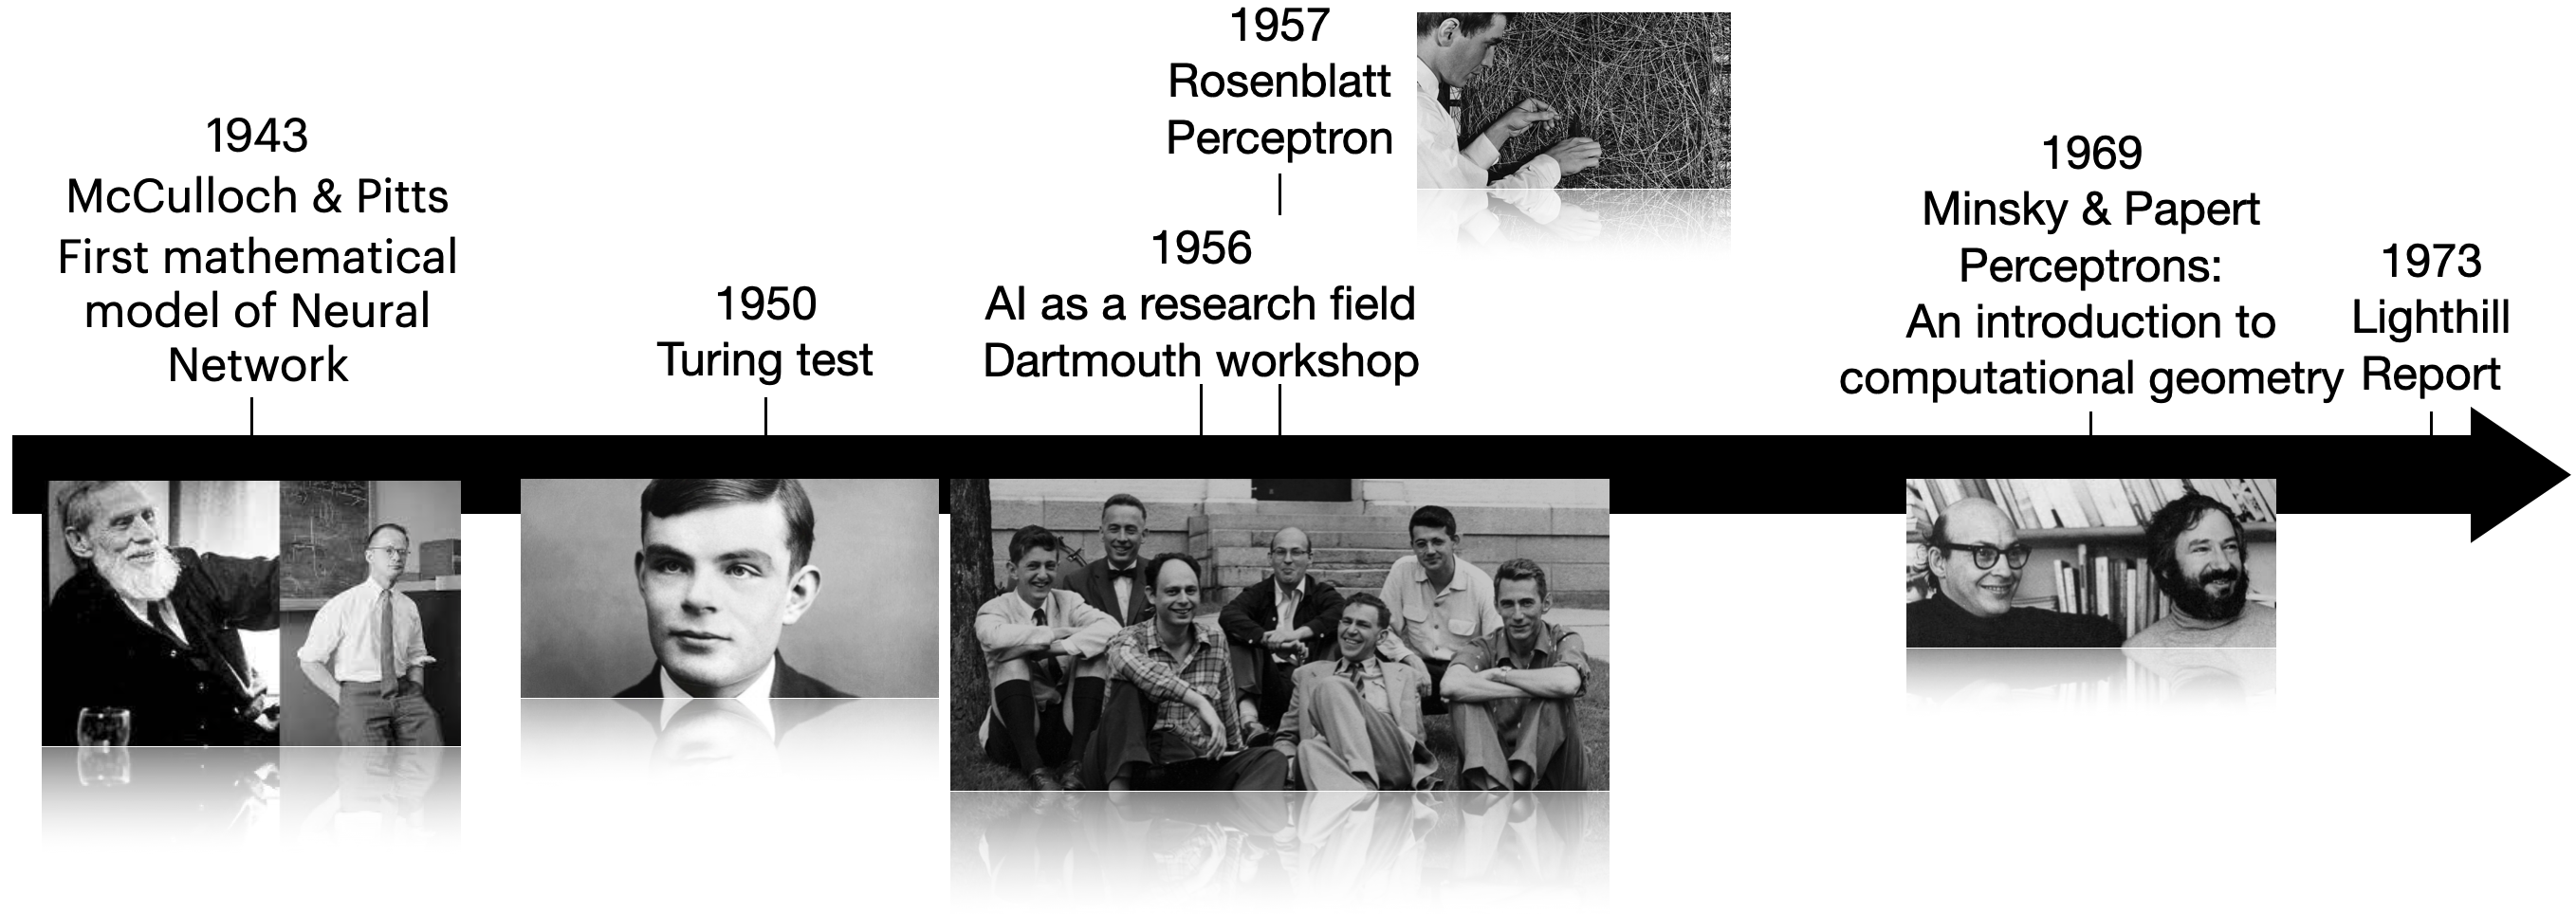
\includegraphics[width=\textwidth]{img/ai_history_1940_1974.png}
  \end{textblock}

  % Résumé de la frise
  \begin{textblock}{50}(0, 50)
    \begin{itemize}
      \item AI (1956)
      \begin{itemize}
      \item \footnotesize Discipline focused on creating systems capable of performing tasks that typically require human intelligence, such as learning, problem-solving and decision-making.
      \end{itemize}
      \item ML (1959)
      \begin{itemize}
        \item \footnotesize Field of AI focused on the development and study of algorithms that can learn from data and generalize to unseen data.
      \end{itemize}
    \end{itemize}
  \end{textblock}

  % Résumé des réalisations
  \begin{textblock}{50}(50, 60)
    \begin{itemize}
      \item Approches symboliques ou non
      \item Réalisations concrètes
    \end{itemize}
  \end{textblock}

\end{frame}


\begin{frame}
  \frametitle{AI winters and expert systems (1974-2000)}

  \begin{textblock}{100}(0,10)
    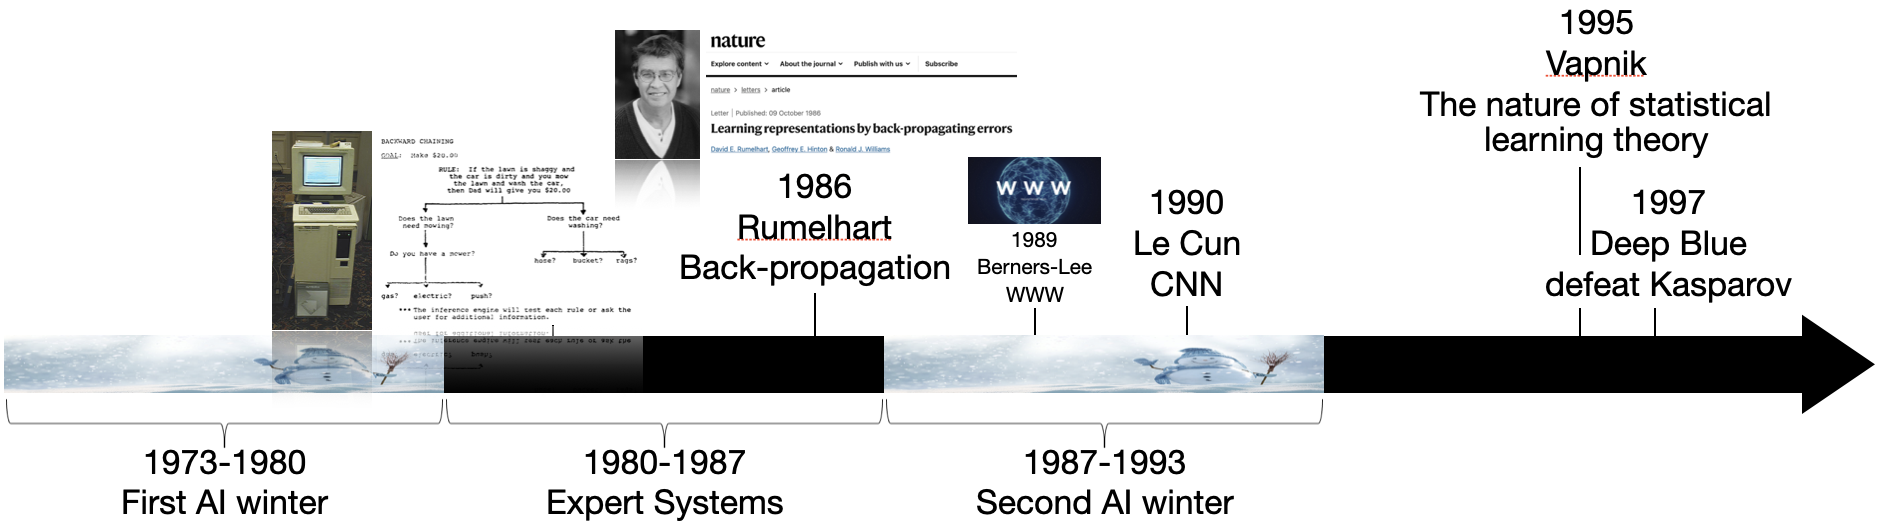
\includegraphics[width=\textwidth]{img/ai_history_1974_2000.png}
  \end{textblock}

  % Résumé de la frise
  \begin{textblock}{50}(0, 60)
    \begin{itemize}
      \item Lighthill report (1973):
      \begin{itemize}
      \item <REF>
      \item Start of the First Winter
      \end{itemize}
      \item Proliferation of expert systems (1980s):
      \begin{itemize}
      \item Symbolic AI
      \item Start of the Second Winter
      \end{itemize}
    \end{itemize}
  \end{textblock}

  % Enseignements, causes, etc.
  \begin{textblock}{50}(50, 60)
    \begin{itemize}
      \item Interesting work in the era:
      \begin{itemize}
      \item Web
      \item Python
      \item Premise of deep learning
      \end{itemize}
      \item Things happen during winter
    \end{itemize}
  \end{textblock}

\end{frame}



\begin{frame}
  \frametitle{Rise Machine Learning and Deep Learning (2000-2024)}

  \begin{textblock}{100}(0,10)
    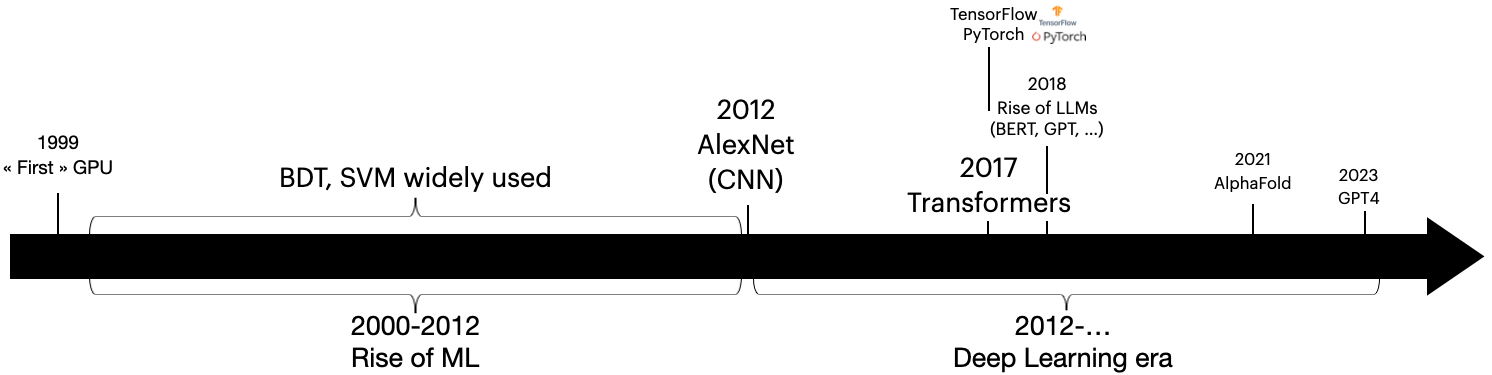
\includegraphics[width=\textwidth]{img/ai_history_2000_2024.png}
  \end{textblock}

  \begin{textblock}{50}(0, 60)
    \begin{itemize}
      \item Big boom
      \item Rise of ML in the early 2000s
      \item AlexNet 2012 CNN
      \item Transformers 2017 leads to first LLMs (2018)
  \end{itemize}
  \end{textblock}

  % Enseignements, causes, etc.
  \begin{textblock}{50}(50, 60)
    \begin{itemize}
      \item TODO
    \end{itemize}
  \end{textblock}

\end{frame}

\subsection{How to go further?}

\begin{frame}
  \frametitle{General books}

  \nocite{*}

  \begin{block}{AI}<1->
    \printbibliography[heading=none,category=AI]
  \end{block}

  \begin{block}{\ac{ML}}<2->
    \printbibliography[heading=none,category=ML]
  \end{block}
\end{frame}

\begin{frame}
  \frametitle{Deep learning books}

  \nocite{*}

  \printbibliography[heading=none,category=deep_learning]
\end{frame}

\begin{frame}
  \frametitle{Courses \& tutorials}

  \begin{block}{Courses}<1->
    \begin{itemize}
    \item Coursera MOOC:
      \url{https://www.coursera.org/specializations/machine-learning-introduction} (more or less based on \href{https://cs230.stanford.edu/}{Stanford CS230 (Deep Learning)})
    \item FIDLE (Formation Introduction au Deep LEarning): \url{https://fidle.cnrs.fr/}
      (yearly course with practical examples in French)
    \end{itemize}
  \end{block}

  \begin{block}{Challenges}<2->
    \begin{itemize}
    \item Kaggle: \url{https://www.kaggle.com/}
    \item ENS Challenge Data: \url{https://challengedata.ens.fr/}
    \end{itemize}
  \end{block}

  \begin{block}{Tutorials}<3->
    \begin{itemize}
    \item PyTorch tutorials: \url{https://pytorch.org/tutorials/} (in-depth
      tutorials about PyTorch)
    \item scikit-lear tutorials:
      \url{https://scikit-learn.org/stable/user_guide.html} (in depth tutorials
      about scikit-learn)
    \end{itemize}
  \end{block}
\end{frame}
